\documentclass[a4paper,12pt, oneside]{article}

%  Русский язык
\usepackage{cmap}					% Улучшенный поиск русских слов
\usepackage[T2A]{fontenc}			% кодировка
\usepackage[utf8]{inputenc}			% кодировка исходного текста
\usepackage[english,russian]{babel}	% локализация и переносы
\usepackage{pscyr}					% нормальные шрифты

% Колонтитулы
\usepackage{fancybox,fancyhdr}
\usepackage{lastpage}
\fancyhf{}
\fancypagestyle{all}
{
	\fancyhead{}
	\fancyhead[C]{\vspace{-5mm}Контрольная работа 12 Вариант Попов Юрий СКБ-171\vspace{3mm}}
	\fancyfoot{}
	\fancyfoot[C]{\hfill  \thepage  \hfill}
}

% Картинки и графики
\usepackage{wrapfig}
\usepackage{pgfplots}
\pgfplotsset{compat=1.9}

% Ссылки
\usepackage{xcolor}
\usepackage{color,colortbl} % раскраска таблиц
\usepackage[unicode, pdftex]{hyperref}
\definecolor{linkcolor}{HTML}{000000} 	% цвет ссылок
\definecolor{urlcolor}{HTML}{8B000F}	% цвет гиперссылок
\hypersetup{urlcolor=urlcolor, linkcolor=linkcolor, colorlinks=true}

% Размеры
\setlength{\paperwidth}{210mm}
\setlength{\paperheight}{297mm}
\setlength{\textheight}{225mm} 			% высота без колонтитулов
\setlength{\textwidth}{170mm}			% ширина текста
\oddsidemargin=0pt
\setlength{\headheight}{2mm}			% высота колонтитула
\setlength{\headsep}{5mm} 	% от блока текста до верхнего колонтитула
\setlength{\footskip}{10mm}  % от блока текста до нижнего колонтитула

% Математика
\usepackage{amsmath,amsfonts,amssymb,amsthm,mathtools,mathtext} 
\usepackage{latexsym,array,epsfig,wasysym}
\usepackage[all]{xy}
\let\int\varint
\def\Int{\int\limits}
\def\IInt{\iint\limits}
\def\IIInt{\iiint\limits}


\begin{document} % начало документа
	
	
	
	\begin{center}
		{\Huge \textbf{Математическая статистика}}
		\vspace{\baselineskip}
		
		{\huge Домашняя работа № 1 \\}
		\vspace{\baselineskip}
		{\huge Вероятностные распределения}
		\vspace{\baselineskip}
		
		{\large Попов Юрий, СКБ-172}
	\end{center}



\vspace{13mm}%Задача 1
\textit{\textbf{Задание 1.1} Выбор одного дискретного распределения
	и одного непрерывного распределения}
\vspace{13mm}

Из представленных в задании таблиц я выбрал \textbf{Геометрическое} (дискретное) и \textbf{Экспоненциальное}(непрерывное) распределения

\vspace{\baselineskip}

Ссылка на  таблицу: \url{https://clck.ru/JdRWD}

	\vspace{\baselineskip}
{\large Сначала проделаем всё домашнее задание для непрерывного распределения}

\vspace{13mm}%Задача 2
\textit{\textbf{Задание 1.2} Описание основных характеристик распределения}
\vspace{13mm}
\\
	Будем искать мат.ожидание и дисперсию через метод моментов.
	
	\vspace{\baselineskip}
	1)Найдем первый момент:
	$$
	E(X) = M\xi = \int_0^\infty x f(x) dx = \int_0^\infty x \lambda \exp(-\lambda x)dx = [- x \exp(- \lambda x)]_0^\infty + \int_0^\infty \exp(-\lambda x) dx = \frac{1}{\lambda}
	$$
	Первый момент == мат. ожиданию, следовательно математическое ожидание мы нашли
	
	\vspace{\baselineskip}
	2)Найдем второй момент:
	
	$$
	M^2\xi = \int_0^\infty x^2 \lambda \exp(-\lambda x) dx = [-x^2 \exp(-\lambda x)]_0^\infty +\int_0^\infty 2 x \exp(-\lambda x)dx =
	$$ 
	
	$$
	= 0 + [-\frac{2}{\lambda} x \exp(-\lambda x)]_0^\infty + \int_0^\infty \exp(-\lambda x)dx = \frac{2}{\lambda}
	$$
	
	По определению $D(X) = E(X^2) - E(X)^2$
	
	Соответственно, $D(X) = \frac{2}{\lambda} - \frac{1}{\lambda} = \frac{1}{\lambda}$ 
	
	\vspace{\baselineskip}
	3)Найдем производящую функцию моментов:
	
	$$
	\begin{array}{rcl}
	M_x(t) &=& E[\exp(tX)] \\
	\\
	&=& \int_{-\infty}^{+\infty} \exp(tx) f_x(x)dx \\
	\\
	&=& \int_0^\infty \exp(tx) \lambda \exp(-\lambda x)dx\\
	\\
	&=& \lambda \int_0^\infty \exp((t-\lambda) x)dx\\
	\\
	&=&\lambda[\frac{1}{t-\lambda} \exp((t-\lambda) x)]_0^\infty\\
	\\
	&=&\frac{\lambda}{\lambda-t}
	\end{array}
	$$
	\\
	Производящая функция моментов: $M_x(t) = \frac{\lambda}{\lambda-t}$
	
	\vspace{\baselineskip}
	4)Найдем характеристическую функцию:
	
	$$
	\begin{array}{rcl}
	\varphi_x(t) &=& E[\exp(itX)]\\
	\\
	&=&\int_{-\infty}^{+\infty} \exp(itx) f_x(x)dx\\
	\\
	&=&\int_0^\infty \exp(itx) \lambda \exp(-\lambda x)dx\\
	\\
	&=&\lambda \int_0^\infty \cos(tx)\exp(-\lambda x)dx + i\lambda \int_0^\infty \sin(tx)\exp(-\lambda x)dx
	\end{array}
	$$
	Отдельно посчитаем каждый интеграл:
	$$
	\begin{array}{rcl}
	\int_0^\infty \cos(tx)\exp(-\lambda x)dx \\
	\\
	&=&[\frac{1}{t} \sin(tx) \exp(-\lambda x)]_0^\infty - \int_0^\infty \frac{1}{t} \sin(tx)(-\lambda \exp(-\lambda x))dx\\
	\\
	&=&\frac{\lambda}{t} \int_0^\infty \sin(tx) \exp(-\lambda x)dx\\
	\\
	&=&\frac{\lambda}{t}\{[-\frac{1}{t} \cos(tx) \exp(-\lambda x)]_0^\infty - \int_0^\infty (-\frac{1}{t} \cos(tx))(-\lambda \exp(-\lambda x))dx\}\\
	\\
	&=&\frac{\lambda}{t}\left(\frac{1}{t} - \frac{\lambda}{t} \int_0^\infty \cos(tx) \exp(-\lambda x)dx\right)\\
	\\
	&=&\frac{\lambda}{t^2} - \frac{\lambda ^2}{t^2} \int_{0}^{\infty} \cos(tx) \exp(-\lambda x)dx
	\end{array}
	$$
	
	Получаем:
	$$
	\int_0^\infty \cos(tx)\exp(-\lambda x)dx = \frac{\lambda}{t^2} - \frac{\lambda ^2}{t^2} \int_{0}^{\infty} \cos(tx) \exp(-\lambda x)dx
	$$
	
	$$
	(1 + \frac{\lambda^2}{t^2})\int_0^\infty \cos(tx)\exp(-\lambda x)dx = \frac{\lambda}{t^2}
	$$
	
	$$
	\int_0^\infty \cos(tx)\exp(-\lambda x)dx = \frac{\lambda}{(t^2 + \lambda^2)}
	$$
	
	Теперь считаем второй интеграл:
	$$
	\begin{array}{rcl}
	 \int_0^\infty \sin(tx)\exp(-\lambda x)dx\\
	 \\
	 &=&[-\frac{1}{t} \cos(tx) \exp(-\lambda x)]_0^\infty- \int_{0}^{\infty}(-\frac{1}{t} \cos(tx))(-\lambda \exp(-\lambda x))dx\\
	 \\
	 &=&\frac{1}{t} - \frac{\lambda}{t}\{ [\frac{1}{t} \sin(tx)\exp(-\lambda x)]_0^\infty - \int_{0}^{\infty} \frac{1}{t} \sin(tx) (-\lambda \exp(-\lambda x ))dx  \}\\
	 \\
	 &=&\frac{1}{t} - \frac{\lambda}{t} (\frac{\lambda}{t} \int_0^\infty \sin(tx) \exp(-\lambda x)dx)\\
	 \\
	  &=&\frac{1}{t} - \frac{\lambda ^2}{t^2} \int_{0}^{\infty} \sin(tx) \exp(-\lambda x)dx
	 \end{array}
	$$
	
	Получаем:
	
	$$
	\int_0^\infty \sin(tx)\exp(-\lambda x)dx = \frac{1}{t} - \frac{\lambda ^2}{t^2} \int_{0}^{\infty} \sin(tx) \exp(-\lambda x)dx
	$$
	
	$$
	(1 + \frac{\lambda^2}{t^2}) \int_0^\infty \sin(tx)\exp(-\lambda x)dx = \frac{1}{t}
	$$
	
	$$
	\int_0^\infty \sin(tx)\exp(-\lambda x)dx = \frac{t}{t^2 + \lambda^2}
	$$

	Соединяем вместе:
	
	$$
	\begin{array}{rcl}
	\varphi_x(t) &=& \int_0^\infty \cos(tx)\exp(-\lambda x)dx +  i \lambda \int_0^\infty \sin(tx)\exp(-\lambda x)dx\\
	\\
	&=&\frac{\lambda^2}{(t^2 + \lambda^2)} + \frac{i\lambda t}{t^2 + \lambda^2}\\
	\\
	&=&\frac{\lambda}{\lambda - i t}
	\end{array}	
	$$
	
	\vspace{\baselineskip}
	Характеристическая функция: $\varphi_x(t) = \frac{\lambda}{\lambda - i t}$
	

	\vspace{\baselineskip}
	5)Найдем функцию распределения:
	
	Если $x < 0$:(Потому что $x$ не может принимать отрицательные значения)
	$$
	F_x(x) = P(X \le x) = 0
	$$
	
	Если $x > 0$:
	$$
	\begin{array}{rcl}
	F_x(x) &=& P(X \le x)\\
	\\
	&=& \int_{-\infty}^{x}f_x(t)dt\\
	\\
	&=& \int_{0}^{x} \lambda\exp(-\lambda t)dt\\
	\\
	&=&[-\exp(-\lambda t)]_0^x\\
	\\
	&=&-\exp(-\lambda x) + 1
	\end{array}	
	$$
	
	Итого, получаем:
	

	\begin{equation*}
	F_x(x) = 
		\begin{cases}
			0 \text{	,$x < 0$}\\
			1 - \exp(-\lambda x) \text{		,$x \ge 0$}
		\end{cases}
	\end{equation*}
	
	\vspace{\baselineskip}
	Перейдем к графикам:
	\vspace{\baselineskip}\\	
	1)График плотности вероятности:

	\begin{minipage}[h]{0.55\linewidth}
		\center{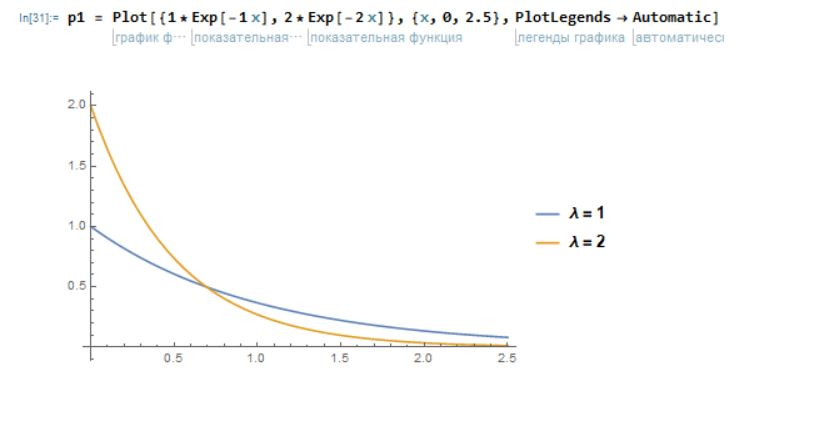
\includegraphics[width=2\linewidth]{1_1.jpg} \\ Рис.1.2.1}
	\end{minipage}
	\\
	\vspace{\baselineskip}\\
	
	2)График функции распределения(при $\lambda = 1$):\\
	\begin{minipage}[h]{0.55\linewidth}	
		\center{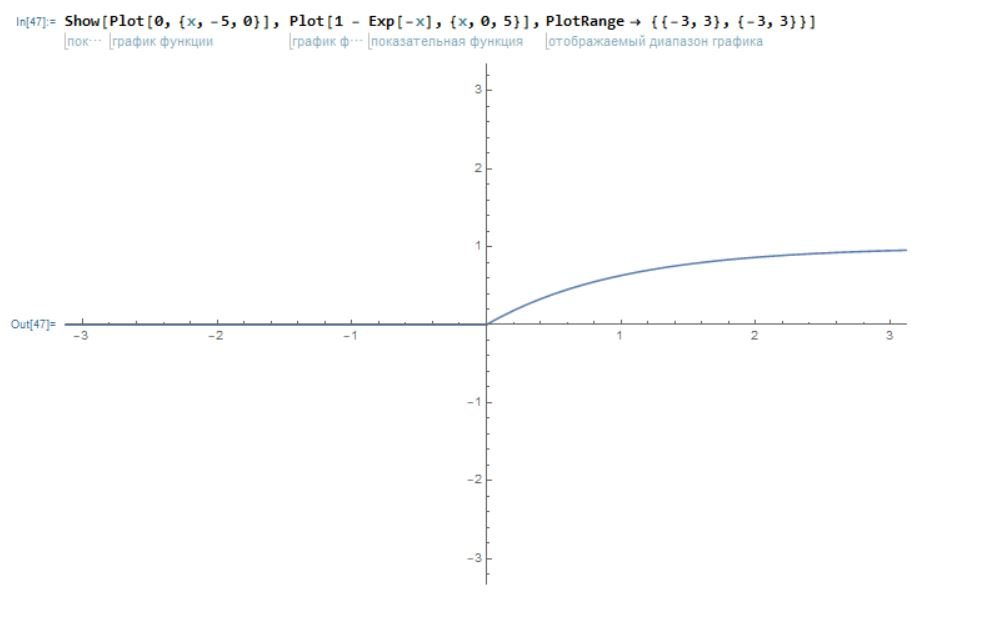
\includegraphics[width=2\linewidth]{1,2,2.jpg} \\ Рис.1.2.2}
	\end{minipage}
	
	
	
	
\vspace{13mm}%Задача 3
\textit{\textbf{Задание 1.3} Поиск примеров событий, которые могут быть описаны выбранными случайными величинами}
\vspace{13mm}


{\bfТипичные интерпретации} экспоненциального распределения:\\
Экспоненциальное распределение в основном используется для тестирования надежности продукта.
Экспоненциальное распределение часто моделирует время ожидания и может помочь вам ответить на такие вопросы, как:

“Сколько времени пройдет, прежде чем сильный ураган обрушится на Атлантическое побережье?” или\\
“Как долго будет работать трансмиссия в моей машине, прежде чем она сломается?".

\vspace{\baselineskip}
Экспоненциальное распределение связано с несколькими известными распределениями.
Информация взята из следующих источников:\\
\href{https://www.statisticshowto.datasciencecentral.com/exponential-distribution/}{Источник1}\\
\href{https://towardsdatascience.com/what-is-exponential-distribution-7bdd08590e2a}{Источник2}
\vspace{\baselineskip}\\
1)Первое это,конечно же, связь с распределением Пуассона:
Если число событий в единицу времени следует распределению Пуассона, то количество времени между событиями следует экспоненциальному распределению. 

Экспоненциальное распределение связано с распределением Пуассона. В то время как экспоненциальная модель моделирует время между последовательными событиями на непрерывном временном интервале, распределение Пуассона имеет дело с событиями, которые происходят в течение фиксированного периода времени. 

\vspace{\baselineskip}
2)Экспоненциальное распределение  является частным случаем гамма-распределения. Это непрерывный аналог геометрического распределения, которое моделирует время между успехами в серии независимых испытаний.

\vspace{\baselineskip}
3)Экспоненциальное распределение также является частным случаем распределения Вейбулла, которое происходит, когда параметр формы Вейбулла = 1.

\vspace{\baselineskip}
4)Связь с распределением Эрланга

Время обслуживания агентов(например, сколько времени требуется сотруднику, чтобы обслужить клиента) также можно смоделировать как экспоненциально распределенные переменные.
Общая длина процесса(последовательность из нескольких независимых задач) следует распределению Эрланга: распределение суммы нескольких независимых экспоненциально распределенных переменных


\vspace{\baselineskip}
{\bfНетипичные интерпретации} экспоненциального распределения:\\
Это также важное распределение для построения непрерывных цепей Маркова.

\vspace{13mm}%Задача 4
\textit{\textbf{Задание 1.4} Описание способа моделирования выбран-
	ных случайных величин}
\vspace{13mm}


{\large Теперь проделаем тоже самое для геометрического распределения!}
\vspace{\baselineskip}
\vspace{\baselineskip}

\vspace{13mm}%Задача 2
\textit{\textbf{Задание 1.2} Описание основных характеристик распределения}
\vspace{13mm}


Будем искать мат.ожидание и дисперсию через метод моментов.

\vspace{\baselineskip}
1)Найдем первый момент:
$$
\begin{array}{rcl}
E[X] &=& \sum\limits_{x=0}^{\infty} (1-p)^x px \\
\\
&=&(1-p)p \sum\limits_{x=0}^{\infty} (1-p)^{x-1} x\\
\\
&=&-(1-p)p \sum\limits_{0}^{\infty} \frac{d}{dp} (1-p)^x\\
\\
&=&-(1-p)p \frac{d}{dp} \sum\limits_{0}^{\infty} (1-p)^x\\
\\
&=&-(1-p)p\frac{d}{dp} \frac{1}{1-(1-p)}\\
\\
&=&-(1-p)p\frac{d}{dp} \frac{1}{p}\\
\\
&=&-(1-p)p(-p^{-2})\\
\\
&=&(p-p^2)p^{-2}\\
\\
&=&\frac{1}{p} - 1\\
\\
&=& \frac{1-p}{p}
\end{array}
$$

Математическое ожидание: $E[X] = \frac{1-p}{p} $


2) Найдем второй момент:
$$
\begin{array}{rcl}
E[X^2] &=& \sum\limits_{0}^{\infty} (1 - p)^x px^2\\
\\
&=&(1-p)^2 p \sum\limits_{x=0}^{\infty} (1-p)^{x-2}x^2\\
\\
&=&(1-p)^2 p \sum\limits_{x=0}^{\infty} (1-p)^{x-2}x (x + 1 -1)\\
\\
&=&(1-p)^2 p \sum\limits_{x=0}^{\infty} (1-p)^{x-2}x (x -1) + \sum\limits_{x=0}^{\infty} (1-p)^{x}x \\
\\
&=&(1-p)^2 p  \sum\limits_{x=0}^{\infty} \frac{d^2}{dp^2}(1-p)^x + E[X]\\
\\
&=& (1-p)^2 p \frac{d^2}{dp^2} \sum\limits_{x=0}^{\infty} (1-p)^x + \frac{1-p}{p}\\
\\
&=&(1-p)^2 p \frac{d^2}{dp^2} \frac{1}{1-(1-p)} + \frac{1-p}{p}\\
\\
&=& (1-p)^2 p \frac{d^2}{dp^2} \frac{1}{p} + \frac{1-p}{p}\\
\\
&=& 2(1-p)^2 p\cdot p^{-3} + \frac{1-p}{p}\\
\\
&=&2(1-2p+p^2)p^{-2} + \frac{1-p}{p}\\
\\
&=&\frac{2 - 3p + p^2}{p^2}
\end{array}
$$

По определению $D(X) = E(X^2) - E(X)^2$

Соответственно,
$$
\begin{array}{rcl}
D(X) &=&\frac{2 - 3p+p^2}{p^2} - ({1-p}{p})^2\\
\\
&=&\frac{2-3p+p^2 -(1-2p + p^2)}{p^2}\\
\\
&=&\frac{1-p}{p^2}
\end{array}
$$

Итого, $D(X) = \frac{1-p}{p^2} $



3)Найдем производящую функцию моментов:

$$
\begin{array}{rcl}
M_x(t) &=& E[\exp(tX)] \\
\\
&=&\sum\limits_{0}^{\infty} (1 - p)^x p \exp(tx)\\
\\
&=& p \sum\limits_{0}^{\infty} [(1 - p)  \exp(t)]^x\\
\\
&=& \frac{p}{1-(1-p)\exp|(t)}
\end{array}
$$

Но у нас есть условие на t :\\
\vspace{\baselineskip}
$(1 - p)  \exp(t) < 1 $
\vspace{\baselineskip}
$\exp(t) < \frac{1}{1-p}$
\vspace{\baselineskip}
$t < -\ln(1-p)$


Итого, производящая функция моментов геометрического распределения определена для $t < -\ln(1-p)$ и равна:
$$
M_x(t) = \frac{p}{1-(1-p)\exp|(t)}
$$


\vspace{\baselineskip}
4)Найдем характеристическую функцию:
$$
\begin{array}{rcl}
\varphi_x(t) &=& E[\exp(itX)]\\
\\
&=&\sum\limits_{0}^{\infty} (1-p)^x p \exp(itx)\\
\\
&=&p \sum\limits_{0}^{\infty} [(1-p)\exp(it)]^x\\
\\
&=&\frac{p}{1-(1-p)\exp(it)}
\end{array}
$$

Итого, характеристическая функция равна:
$$
\varphi_x(t) = \frac{p}{1-(1-p)\exp(it)}
$$

\vspace{\baselineskip}
5)Найдем функцию распределения:

При $x < 0 : F_x(x) = 0$
При  $x > 0: $\\
$$
\begin{array}{rcl}
F_x(x) &=& P(X < x)\\
\\
&=&\sum\limits_{y=0}^x (1 - p)^y p\\
\\
&=&p \sum\limits_{y=0}^x (1 - p)^y\\
\\
&=&p \frac{1 - (1 - p)^{x + 1}}{1 - (1 - p)}\\
\\
&=& 1 - (1 - p)^{x + 1}
\end{array}
$$

Итого, функция распределения равна:
\begin{equation*}
F_x(x) = 
\begin{cases}
0 \text{	,    $x < 0$}\\
1 - (1 - p)^{x + 1} \text{		,      $x \ge 0$}
\end{cases}
\end{equation*}

\vspace{\baselineskip}
Перейдем к графикам:
\vspace{\baselineskip}\\	
1)Гистограмма вероятностей($p = 1/6$):

\begin{minipage}[h]{0.55\linewidth}
	\center{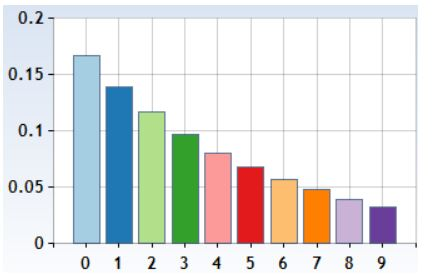
\includegraphics[width=1\linewidth]{1,4.jpg} \\ Рис.1.2.3}
\end{minipage}
\\
\vspace{\baselineskip}\\

2)График функции распределения:\\
\begin{minipage}[h]{0.55\linewidth}	
	\center{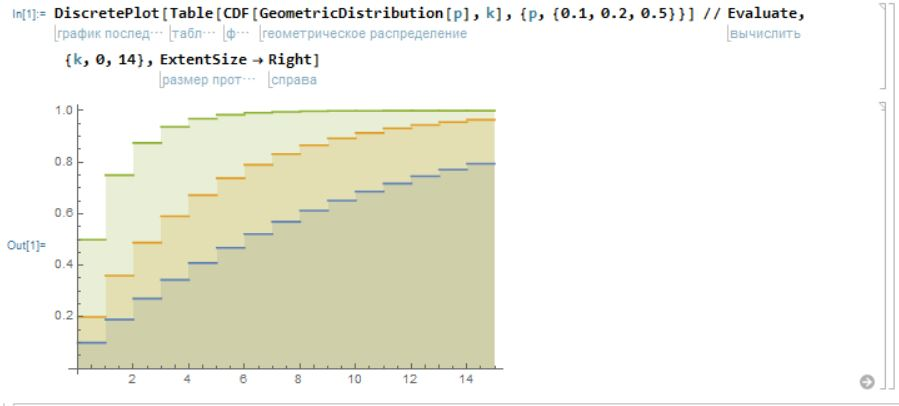
\includegraphics[width=2\linewidth]{1,3,1.jpg} \\ Рис.1.2.4}
\end{minipage}















\end{document}

